% AI stuff
\newcommand{\domain}{\mathds{D}}
\newcommand{\entities}{\texttt{ent}}
\newcommand{\consistsWith}{\texttt{cw}}
\newcommand{\charFunML}{\charactheristicFunction}
\newcommand{\aCircuit}{\mathcal{C}}

% Computational complexity stuff
\newcommand{\NP}{\textsc{NP}}
\newcommand{\NPhard}{\textsc{NP-hard}}
\newcommand{\NPcomplete}{\textsc{NP-complete}}
\newcommand{\sharpPhard}{\textsc{\#P-hard}}

% Sets and probability stuff
\newcommand{\R}{\mathds{R}}
\newcommand{\perm}{perm}
\newcommand{\aDistribution}{\mathcal{D}}
\newcommand{\expectancy}{\mathds{E}}
% Important names and stuff
\newcommand{\SHAPscore}{\textsc{SHAP-score}}
\newcommand{\aBayesianDistribution}{\mathcal{B}}
\newcommand{\set}[1]{ \{ #1 \} }

% Game Theory
\newcommand{\charactheristicFunction}{\nu}
\newcommand{\players}{\mathcal{I}}
\newcommand{\Shap}{Shap}
\newcommand{\assym}{\Shap^{assym}}

% DAG and Assym Notation
\newcommand{\toOr}{\pi} %topologicalOrder
\newcommand{\rel}{R} %relation
\newcommand{\union}{union}
\newcommand{\equivalenceClass}{[\pi]_{\rel}} %equivalenceClass
\newcommand{\eqClassSize}{eqClassTopos}
\newcommand{\equivalenceClassRep}{\mathsf{Rep}(\equivalenceClass)}
\newcommand{\numEqCl}{\#EC} %equivalenceClass formula
\newcommand{\unrEqCl}{UnrEC} %unrelated equivalenceClass formula
\newcommand{\heuristicASVFormula}{\frac{1}{|\topo(G)|} \sum_{\equivalenceClass \in eqCl(G, x_i)} (\charactheristicFunction(\toOr_{<i} \cup \{x_i\}) - \charactheristicFunction(\toOr_{<i})) * |\equivalenceClass|} %New Formula
\newcommand{\eqClassSizes}{eqClassSizes} %unrelated equivalenceClass sizes formula
\newcommand{\leftPossibleOrders}{\#LO} %Left possible orders

%% Drawing graphs

\newcommand{\drawUnrelatedTreeWithColor}[5]{
    \node[circle, draw=#5] (#1) at (#2, #3) {#4};
    \pgfmathsetmacro{\x}{#2-2}
    \pgfmathsetmacro{\y}{#3-0.3} 
    \draw[#5, wiggly] (#2, \y)
        -- ++(-1,-1.6) 
        -- ++(2,0) 
        -- cycle;
    \node[text=#5, font=\Large] at (\x, \y) {#4 subárbol};
}

\newcommand{\drawUnrelatedTree}[4]{
    \drawUnrelatedTreeWithColor{#1}{#2}{#3}{#4}{red}
}

\newcommand{\drawUnrelatedTreeWithTag}[6]{
    \drawUnrelatedTreeWithColor{#1}{#2}{#3}{#4}{#5}

    % Texto de nodos disponibles (más abajo del contorno)
    \pgfmathsetmacro{\ysubtree}{#3 - 0.3}
    \pgfmathsetmacro{\ytext}{\ysubtree - 2.0}
    \node[font=\Large, text=#5] at (#2, \ytext) {#6};
}

\newcommand{\drawUnrelatedTreeLarge}[4]{%
	% Nodo grande
	\node[circle, draw=red, minimum size=1.5cm, inner sep=3pt, font=\Large] 
	(#1) at (#2,#3) {#4};%
	% Wiggly inferior (ajustar offsets si es necesario)
	\pgfmathsetmacro{\yy}{#3-0.8}%
	\draw[red,wiggly,line width=1pt] 
	(#2,\yy) 
	-- ++(-1.2,-2) 
	-- ++(2.4,0) 
	-- cycle;%
}

% Graphs and networks
\newcommand{\topo}{topos}
\newcommand{\numTopo}{\#topos}
\newcommand{\aBayesianNetwork}{N}
\newcommand{\parents}{\textit{Parents}}
\newcommand{\dtrees}{\emph{dtrees}}
\newcommand{\dtree}{\emph{dtree}}
\newcommand{\childNetwork}{\emph{Child}}
\newcommand{\cancerNetwork}{\emph{Cancer}}
\newcommand{\variableNetwork}[1]{\texttt{#1}}
\newcommand{\intersectionNode}{i_{\cap}}
\newcommand{\subtree}{s}

%Redefiniendo environments
\newtheorem{myexample}{Ejemplo}
\newtheorem{mytheorem}{Teorema}
\newtheorem{myproposition}{Proposición}
\newtheorem{mylemma}{Lema}
\newtheorem{mycorollary}{Corolario}
\newtheorem{myobservation}{Observación}
\newtheorem{mysketch}{Boceto}
\newtheorem{myacknowledgements}{Agradecimientos}
\newtheorem{mydefinition}{Definición}

%Definiciones varias

\def\cmd#1{\texttt{\color{red}\footnotesize $\backslash$#1}}
\def\env#1{\texttt{\color{blue}\footnotesize #1}}
\definecolor{deepblue}{rgb}{0,0,0.5}
\definecolor{ccnuMainColor}{RGB}{0,86,109}
\definecolor{deepgreen}{rgb}{0,0.5,0}
\definecolor{halfgray}{gray}{0.55}

\lstset{
    basicstyle=\ttfamily\small,
    keywordstyle=\bfseries\color{deepblue},
    emphstyle=\ttfamily\color{ccnuMainColor},    % Custom highlighting style
    stringstyle=\color{deepgreen},
    numbers=left,
    numberstyle=\small\color{halfgray},
    rulesepcolor=\color{red!20!green!20!blue!20},
    frame=shadowbox,
}

\newtcolorbox{myblock}[1]{
  colback=halfgray!20, 
  colframe=ccnuMainColor, 
  fonttitle=\bfseries, 
  title=#1, 
  rounded corners
}

\newcommand{\dificultyLevel}[1]{ %To add the voleyball slides representing the difficulty level
%1 -> Apto para toda la familia
%2 -> Escuchame y llegas
%3 -> Hay que saber de grafos y prestar atención
  \begin{tikzpicture}[remember picture,overlay]
    \foreach \i in {1,...,#1} {
      \node[anchor=north east, yshift=-16pt, xshift={-1.5em*\i}] at (current page.north east) {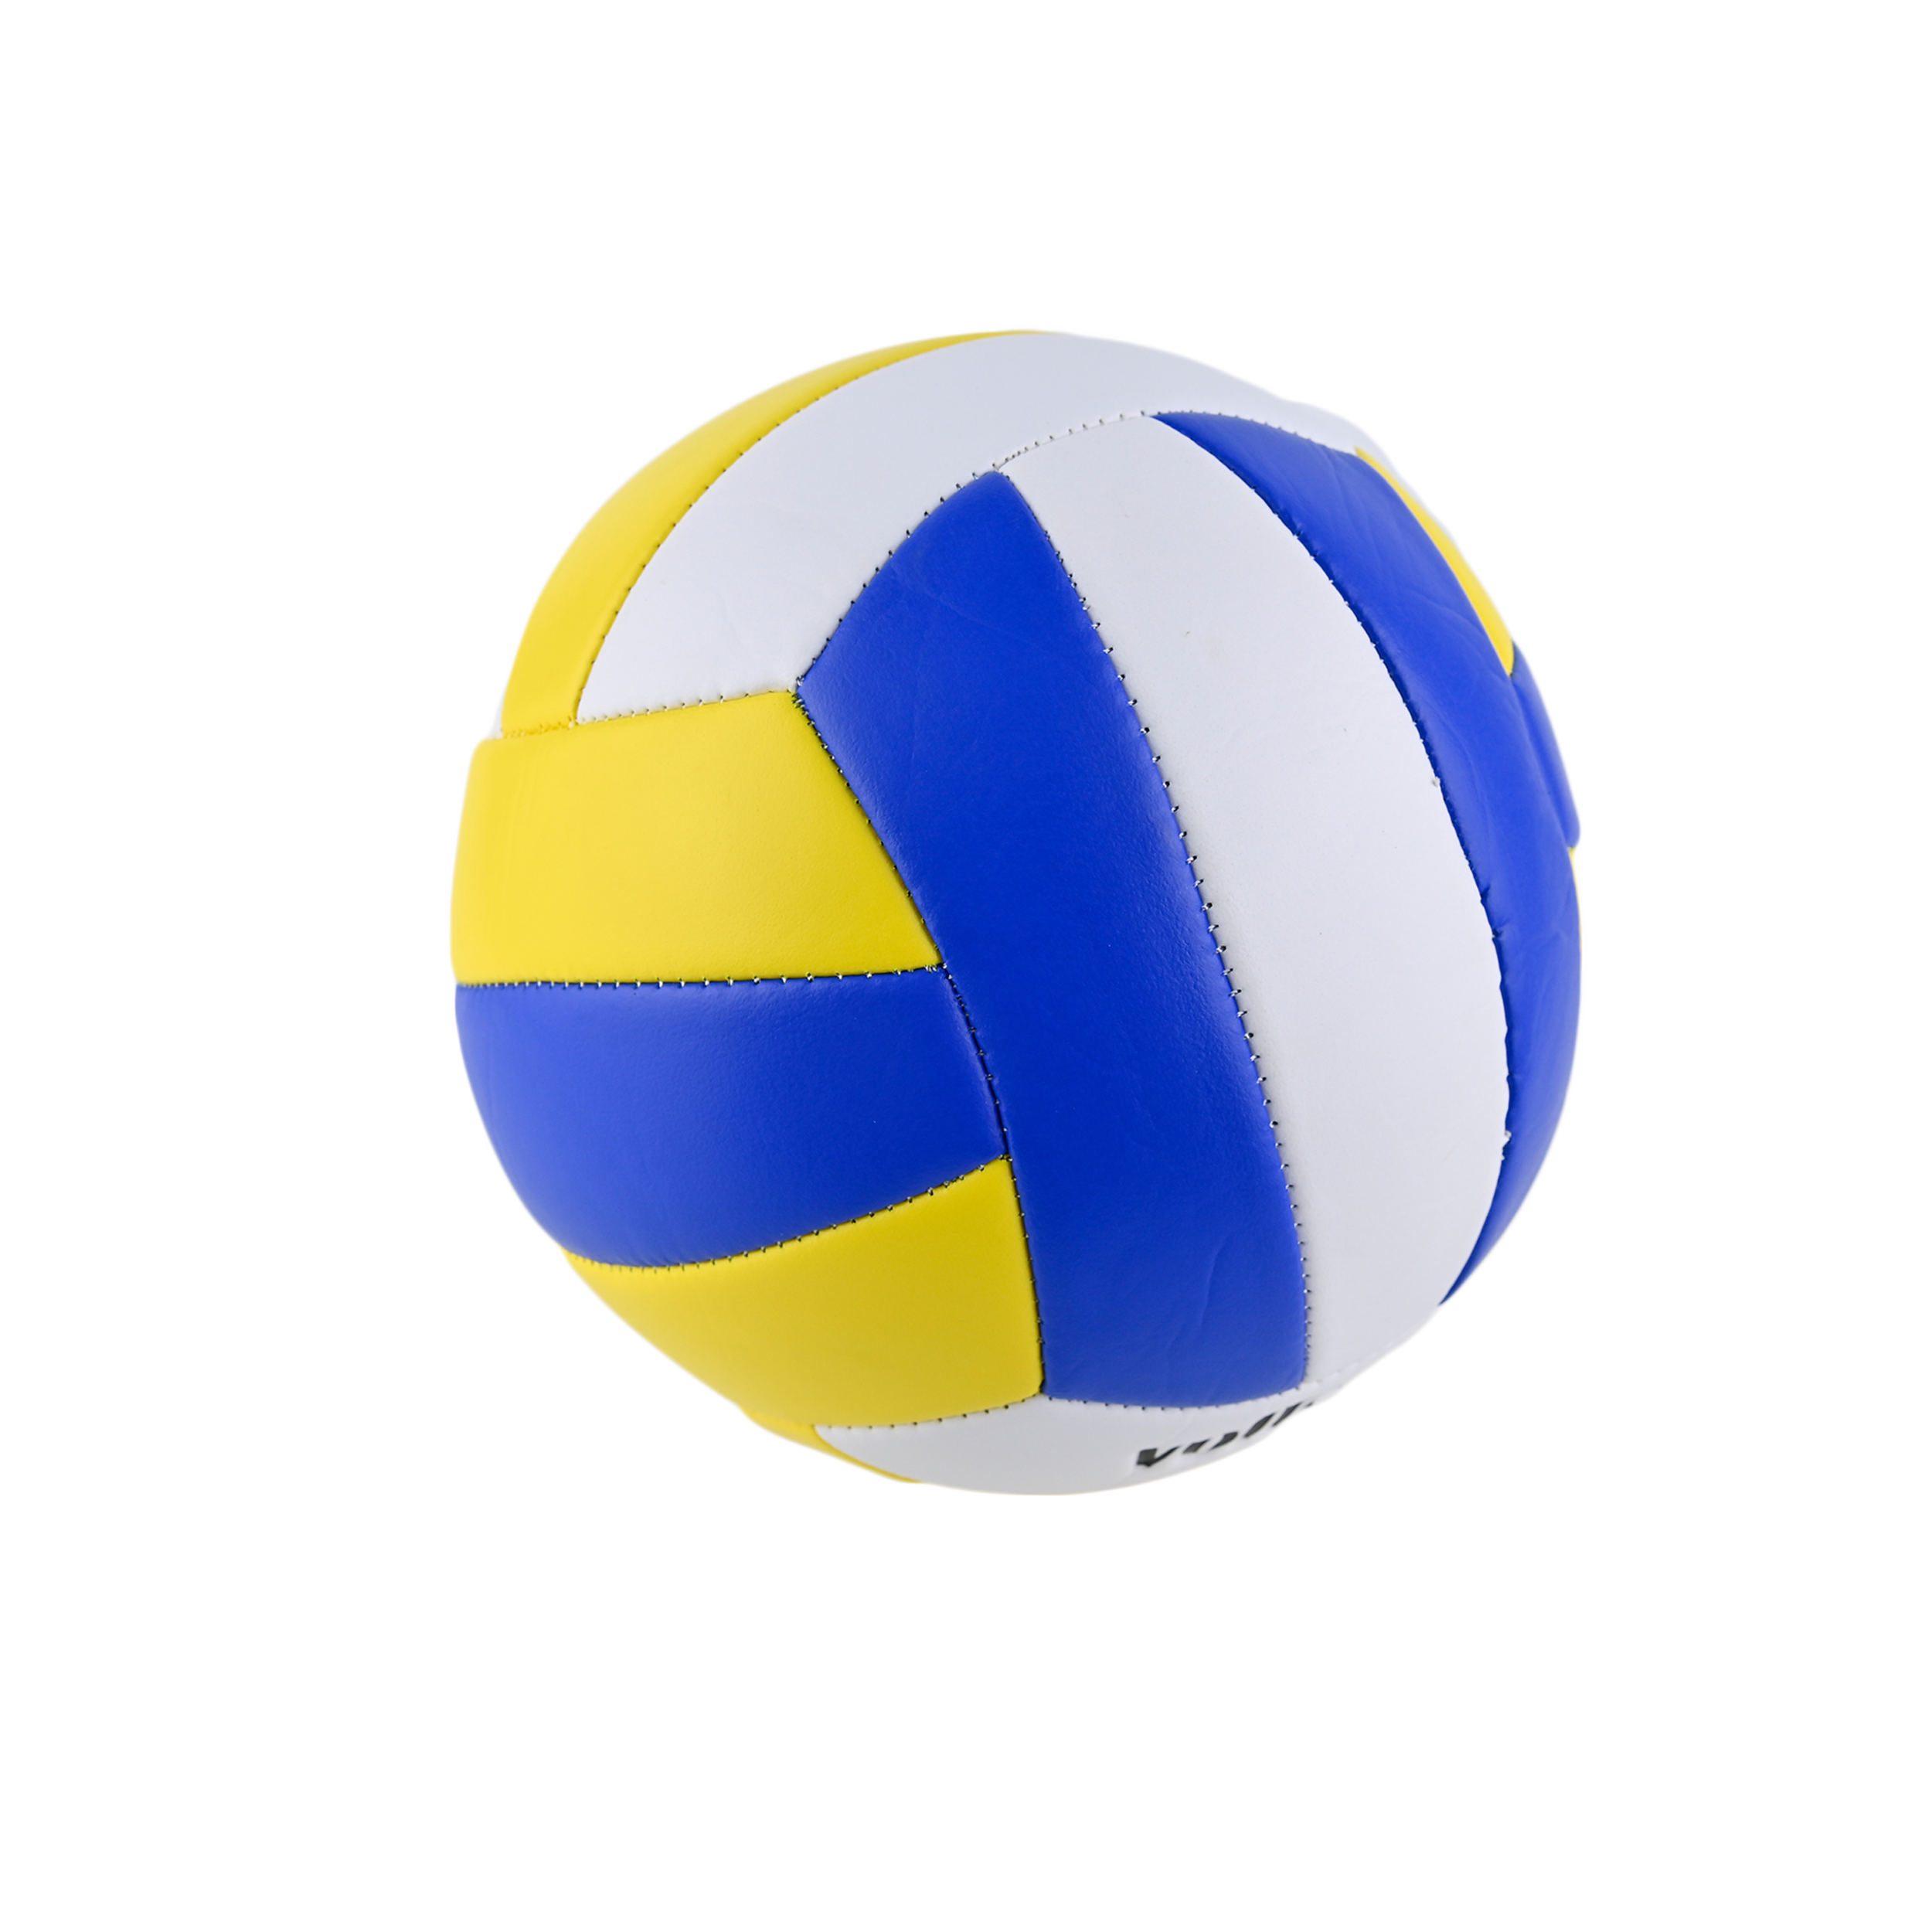
\includegraphics[width=2em]{pic/voleyball.png}};
    }
  \end{tikzpicture}%
}